\documentclass[../main.tex]{subfiles}

\begin{document}
	\subsection{$I_{DS}$ function of $V_{DS}$}
	{
		\begin{tcolorbox}[colback=gray!5!white,colframe=gray!75!black]
			Plot, for the two types of transistors, the graph $I_{DS}(V_{DS}, V_{GS})$ for $V_{GS}$ constant, and for $V_{DS}$ varying between between $V_{SS}$ and $V_{DD}$. These plots will be done for several values of $V_{GS}$. Identify the linear and saturation domains for both types of transistors.
		\end{tcolorbox}
		
	
		\subsubsection{NMOS transistor}
		{
			
		We will use $V_{GS}$ equal to $1V$, $2V$ and $3V$ (so we are never in the cutoff region because $V_{GS} > V_{tn}$).
			
		Theoretically we expect
		
		\begin{equation}
			I_{DS}(V_{DS}, V_{GS} = \text{constant}) = 
			\begin{cases} 
				k_n \frac{W}{L} \left[(V_{GS} - V_{tn})V_{DS} - \frac{V_{DS}^2}{2}\right], & \text{if } V_{DS} < V_{GS} - V_{tn} \text{ (triode or linear)}, \\[5pt]
				\frac{1}{2} k_n \frac{W}{L} (V_{GS} - V_{tn})^2, & \text{if } V_{GS} \geq V_{tn} \text{ (saturation)}.
			\end{cases}
		\end{equation}
		
		\begin{lstlisting}
			.include cmosws.mod
			
			Vds 2 0 dc 3.3V
			Vgs 1 0 dc 1V
			M1  2 1 0 0 MODN L=0.6U W=3.0U
			
			.dc Vds 0 3.3 50mV Vgs 1 3 1V
			.end
		\end{lstlisting}
		
		\begin{figure}[H]
			\centering
			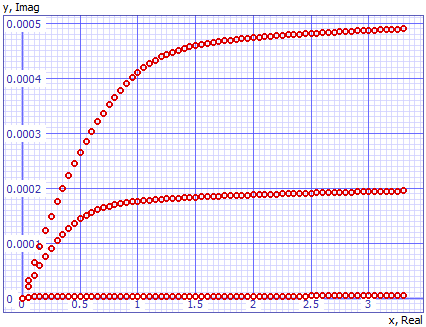
\includegraphics[width=0.5\textwidth]{plots/Q2_nmos.png}
			\caption{$I_{DS}$ function of $V_{DS}$ for NMOS transistor}
		\end{figure}
		
		}
		
		\subsubsection{PMOS transistor}
		{
			
		Once again for the PMOS, we make adaptions to account for reversed polarity.
		
		We will use $V_{SG}$ equal to $1V$, $2V$ and $3V$ (so we are never in the cutoff region because $V_{SG} > |V_{tp}|$).
		
		Theoretically we expect
		
		\begin{equation}
			I_{DS}(V_{SD}, V_{SG} = \text{constant}) = 
			\begin{cases} 
				-k_p \frac{W}{L} \left[(V_{SG} - |V_{tp}|)V_{SD} - \frac{V_{SD}^2}{2}\right], & \text{if } V_{SD} < V_{SG} - |V_{tp}| \text{ (triode or linear)}, \\[5pt]
				-\frac{1}{2} k_p \frac{W}{L} (V_{SG} - |V_{tp}|)^2, & \text{if } V_{SG} \geq |V_{tp}| \text{ (saturation)}.
			\end{cases}
		\end{equation}
		
		\begin{lstlisting}
			.include cmosws.mod
			
			Vsd 2 0 dc 3.3V
			Vsg 2 1 dc 1V
			M1  0 1 2 2 MODP L=0.6U W=6.0U
			
			.dc Vsd 0 3.3 50mV Vsg 1 3 1V
			.end
		\end{lstlisting}
		
		\begin{figure}[H]
			\centering
			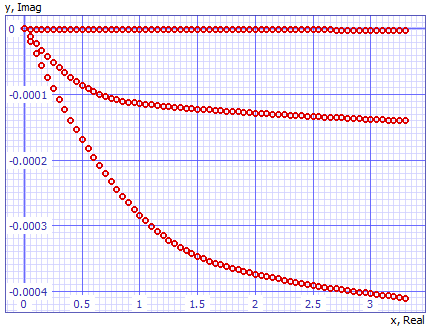
\includegraphics[width=0.5\textwidth]{plots/Q2_pmos.png}
			\caption{$I_{DS}$ function of $V_{SD}$ for PMOS transistor}
		\end{figure}
	
		}
	}
	
\end{document}